\Section{Network Setup}

In this chapter the cINN setup will be discussed. In the first half, the generation of training and test datasets is going to elaborated, with a detailed focus on the analysis specifics, such as interpolation between histograms (morphing) and the representation of the statistic and systematic uncertainties.

In the second half of this chapter, the final cINN architecture used for the inference is going to be presented. The results of the inference and the interpretation of the network outputs will be discussed in the next chapter.

\Subsection{Training Dataset Generation}

The conditions shown in fig \ref{fig:conditions} in chapter \ref{ch:analysis_strategy} represent the expectation on the measured dataset. Unfortunately, the share of each process in each bin in the measured data is a priori unknown (which would mean the complete physics is known to the very last detail). For this purpose the different scenarios of a process having more or less shares in a bin have to be first artificially represented in the dataset in order to obtain a cINN which is capable of inferring the share of each process -- or in other words, to obtain the signal modifier parameters $\mu_i$.

\Subsubsection{Prior Selection}

In order to do so, a set of signal modifier parameters are drawn from a pool of expected parameter distribution (the prior). Then, each process in the histogram is scaled with the corresponding parameter and the bins will summed up meaning (similar to the expected dataset) the information about the contribution of each process to each bin is lost.

The prior distribution for the processes have been selected as the following. For the signal processes \texttt{ggZH}, \texttt{ZHDY} and \texttt{WH} the $\mu_i$ were sampled from a gamma distribution

\begin{equation*}
	f(x; k, \theta) = \frac{x^{k-1}e^{-x/\theta}}{\theta^k\Gamma(k)}
\end{equation*}

with shape parameter $k$ and scale $\theta$. An advantage of this distribution as prior is the positiveness of the samples $\{x_i\}$ from the distribution; apart from that, the distribution has a long tail for increasing values of $x$ which allow a more fined selection in a given range. The parameters were set to be $k = 1.5$ and $\theta = 7$; with this specific selection, one obtains a prior which is sensitive in the low signal yield region $\mu \lesssim 10$ while maintaining network sensitivity for values $\mu<100$.

For the background processes, it is expected that the MC simulations follow the expectation with good accuracy. Hence, one expects $\mu \approx 1$. For this reason, the prior has been chosen to follow a lognormal distribution

\begin{equation*}
	f(x; \mu, \sigma) = \frac{1}{\sqrt{2\pi }\sigma x}\exp\left(-\frac{\left(\ln(x)-\mu\right)^2}{2\sigma^2}\right)
\end{equation*}

with mean $\mu = 0.05$ and $\sigma = 0.25$, lognormal distributions being positive themselves.

In order the estimate the arising uncertainty from the luminosity, the obtained conditions (after scaling and uncertainty variation) are then scaled with an additional luminosity factor. These have been drawn from a lognormal distribution with $\mu = 0$ and $\sigma = 0.02$.
All distributions are shown in fig. \ref{fig:priors}.

\begin{figure}[h!]
	\centering
	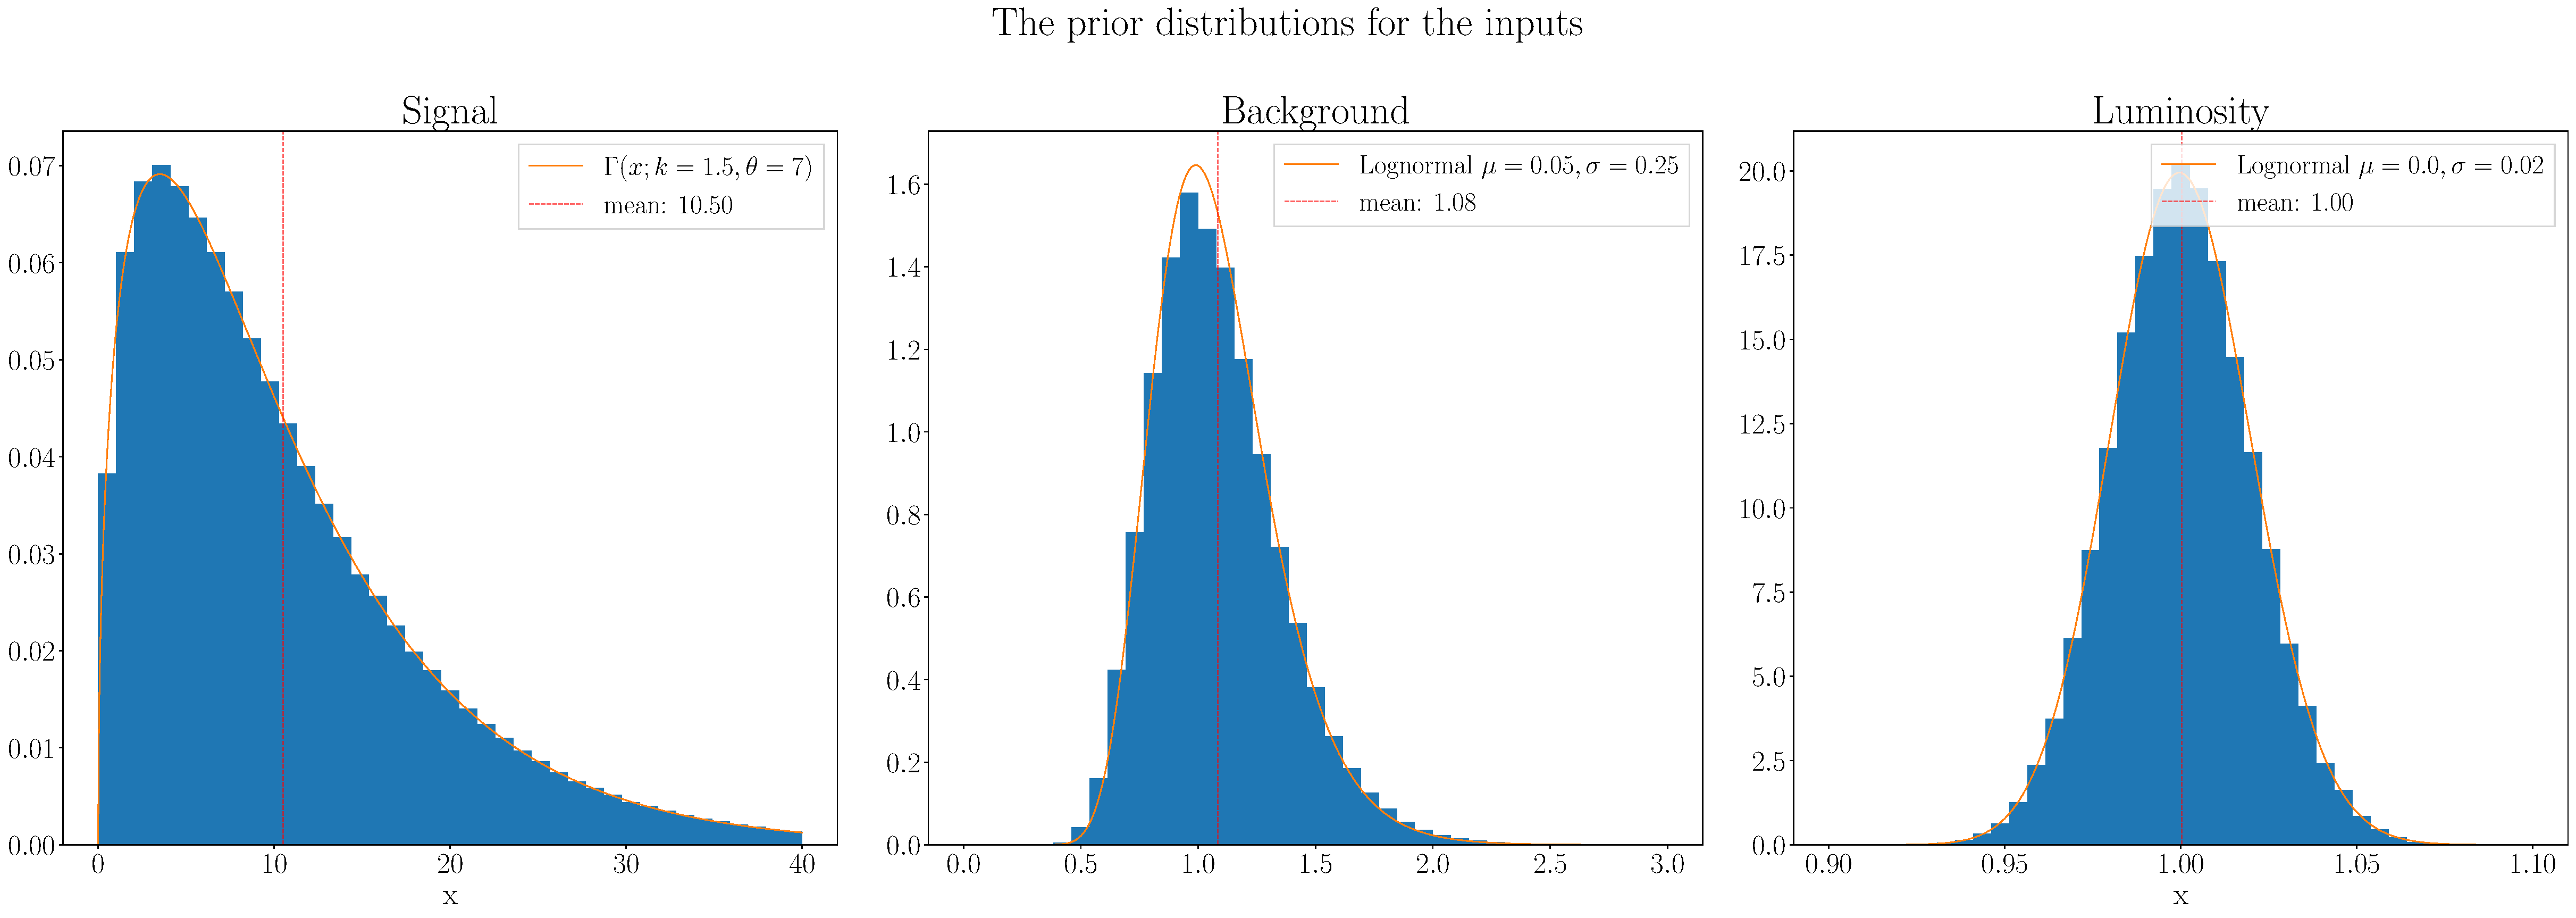
\includegraphics[width=\linewidth]{figures/network_setup/priors.pdf}
%	\begin{minipage}{.5\textwidth}
%		\centering
%%		\includegraphics[width=0.8\linewidth]{figures/network/signal}
%	\end{minipage}%
%	\begin{minipage}{.5\textwidth}
%		\centering
%%		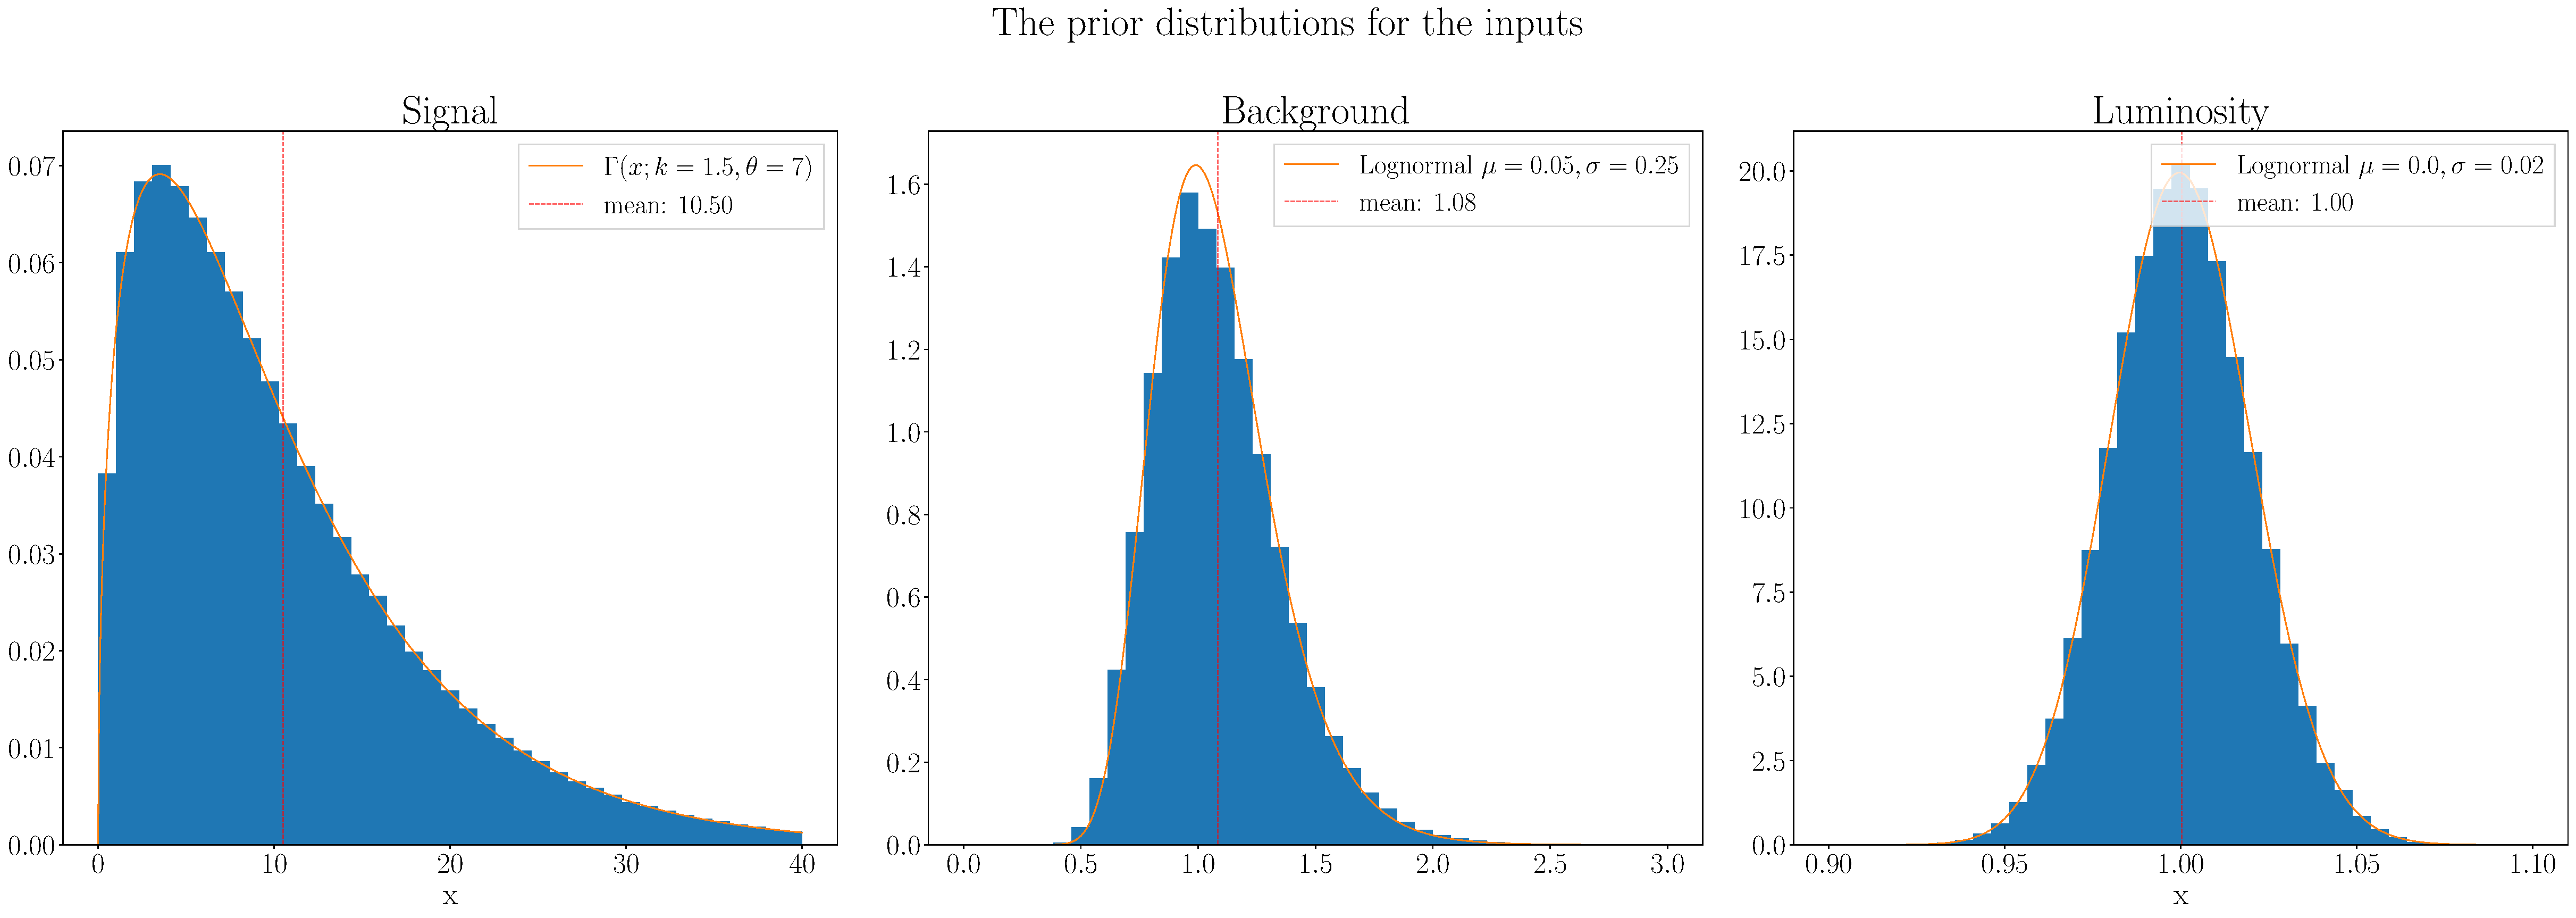
\includegraphics[width=0.6\linewidth]{figures/network_setup/priors.pdf}
%	\end{minipage}
	\caption{Prior distributions for the signal and background processes. Samples are shown in blue; the mean of each distribution is shown with the red dashed line. The analytic shape of each distribution is shown in orange.}
	\label{fig:priors}
\end{figure}

After successful histogram scaling, the statistical and systematic uncertainty fluctuations are applied to the scaled histogram.

\Subsection{Systematic Uncertainties}

\textcolor{red}{There are 24 sources of systematic uncertainties which have been taken into account. These are:} \\

%\begin{tabular}{c}
%	\texttt{PDFSet               }  \\
%	\texttt{PSWeight\_FSR        }  \\
%	\texttt{PSWeight\_ISR        }  \\
%	\texttt{ScaleWeight\_Envelope}  \\
%	\texttt{ScaleWeight\_Fact    }  \\
%	\texttt{ScaleWeight\_Mixed   }  \\
%	\texttt{ScaleWeight\_Renorm  }  \\
%	\texttt{btagWeight\_cferr1   }  \\
%	\texttt{btagWeight\_cferr2   }  \\
%	\texttt{btagWeight\_hf       }  \\
%	\texttt{btagWeight\_hfstats1 }  \\
%	\texttt{btagWeight\_hfstats2 }  \\
%	\texttt{btagWeight\_lf       }  \\
%	\texttt{btagWeight\_lfstats1 }  \\
%	\texttt{btagWeight\_lfstats2 }  \\
%	\texttt{electron\_id         }  \\
%	\texttt{electron\_reco       }  \\
%	\texttt{l1\_ecal\_prefiring  }  \\
%	\texttt{muon\_id             }  \\
%	\texttt{muon\_iso            }  \\
%	\texttt{pileup               }  \\
%%  \texttt{trigger\_e\_sf       }  \\
%	\texttt{trigger\_ee\_sf      }  \\
%	\texttt{trigger\_mu\_sf      }  \\
%	\texttt{trigger\_mumu\_sf    }  \\
%%  \texttt{top\_pT\_reweighting }  \\
%%  \texttt{TuneCP5              }  \\
%\end{tabular} 

The systematic uncertainties require an interpolation method as the shifts in the histograms are computationally expensive to obtain. In other words, as only the effect of the $1\sigma$ up- and down-shifts of the uncertainties (templates) listed above are given, the task to represent the in-between-cases (and obviously, those of outside of the given range) in the histrograms remains. For this purpose, a non-linear histogram morphing method has been implemented.

In the following, an overview of the morphing algorithm will be given with a discussion on the implementation and on its effects on the histograms following thereafter.

\Subsubsection{Non-linear Histogram Morphing}

Non-linear histogram morphing has been implemented on the basis of \cite{Baak_2015}. For the interpolation a nominal distribution and -- in this case -- 24 other distribution templates representing the $1\sigma$ and $-1\sigma$ shifts are given. The nominal template $f(x|m)$ with morphing parameter $m$ can then be appromated around $m=0$ with the other templates in a simple 1D case using

\begin{equation*}
	f(x|m) \approx \sum_j \left.\frac{\partial^{(j)} f(x|m)}{\partial m^{(j)}}\right|_{m=0}\frac{m^j}{j!} = \sum_j f_j'(x|m=0) m^j
\end{equation*}



where the derivatives and the factorials have been absorbed in $f'_j$.

For $T$ uncorrelated uncertainties (hence for $T$ morphing parameters $m$) with morphing parameter values $\pm1$ there are $2T+1$ sampled distributions in total (counting the nominal distribution). An intuitive representation of the "morphing parameter space" with the indication of the available templates is shown in fig. \ref{fig:morphing_phase_space}.

\begin{figure}[h!]
	\centering
	\centering
	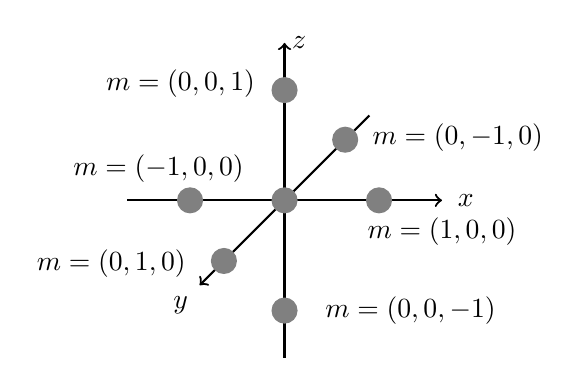
\begin{tikzpicture}[scale=2]
		\coordinate (O) at (0,0,0);
		\draw[thick,->] (-1.,0,0) -- (1.,0,0) node[right=2]{$x$};
		\draw[thick,->] (0,-1,0) -- (0,1,0) node[right=-1]{$z$};
		\draw[thick,->] (0,0,-1.4) -- (0,0,1.4) node[below left=0.5]{$y$};
		
		\node[circle, fill=gray] (0) {};
		\node[circle, fill=gray] at (   0,-0.7, 0) {};
		\node at (0.8, -0.7, 0) {$m=(0,0,-1)$};
		\node[circle, fill=gray] at (   0, 0.7, 0) {};
		\node at (-1.2, 0.2, -1.4) {$m=(0,0,1)$};
		\node[circle, fill=gray] at (   0, 0  ,-1) {};
		\node at (-0.8, 0.2, 0) {$m=(-1,0,0)$};
		\node[circle, fill=gray] at (   0, 0  , 1) {};
		\node at (1, -0.2, 0) {$m=(1,0,0)$};
		\node[circle, fill=gray] at (-0.6, 0  , 0) {};
		\node at (-1.1, -0.4, 0) {$m=(0,1,0)$};
		\node[circle, fill=gray] at ( 0.6, 0  , 0) {};
		\node at (1.1, 0.4, 0) {$m=(0,-1,0)$};
	\end{tikzpicture}
	\caption{The morphing "phase space" showing the available distributions for $T=3$ uncertainties of $\sigma=\pm1$. The available templates in the phase space are shown in grey. Note that the nominal template with $m=(0,0,0)$ lies in the origin and there are no "mixed" templates (such as $m = (1,1,0)$) available. In the setting described above, one has $T=24$, hence there are $24\times2 +1 = 49$ templates in total.}
	\label{fig:morphing_phase_space}
\end{figure}

For theis multidemensional case as there are no "mixed templates" taking into account the effect of two independent systematic variations, the mixed derivative terms from the above expansion are zero. Hence, the expression can be written for a given $\mathbf{m}_i$\footnote{$\mathbf{m}_i = (0, 0, ..., 0, \pm 1, 0, ..., 0)$ for the i-th template with $\sigma=\pm1$} as:

\begin{equation}
	f(x | \mathbf{m}_i) = \underbrace{\vphantom{\frac{1}{2!}\left.\frac{\partial^2 f(x | \mathbf{m})}{\partial m_j^2}\right|_{\mathbf{m}=0}}f(x | 0)}_{f_0} + \sum^T_{j=1} \underbrace{\vphantom{\frac{1}{2!}\left.\frac{\partial^2 f(x | \mathbf{m})}{\partial m_j^2}\right|_{\mathbf{m}=0}}\left.\frac{\partial f(x | \mathbf{m})}{\partial m_j}\right|_{\mathbf{m}=0}}_{f'_j}(m_i)_j + \sum^T_{j=1} \underbrace{\frac{1}{2!}\left.\frac{\partial^2 f(x | \mathbf{m})}{\partial m_j^2}\right|_{\mathbf{m}=0}}_{f'_{jj}}(m_i)^2_j + \mathcal{O}\left((m_i)_j^3\right)
	\label{eq:morphing}
\end{equation}

where $(m_i)_j$ denotes the j-th component of the i-th morphing parameter vector. The aim is to find an expression for the unknown derivatives as only the histogram $f(x|m)$ is given. If one knew the derivatives, one could easily select a general $m_i$ and insert in into eq. \ref{eq:morphing}, yielding the morphed distribution.

In order to express the derivatives write all given templates in a vectorized form, and make use of the matrix form

\begin{equation*}
	\left(\begin{aligned}
		f\Bigl(x &| (0,\phantom{-}0, 0\,,...,\phantom{-}0)\Bigl) \\
		f\Bigl(x &| (0,\phantom{-}1, 0\,,...,\phantom{-}0)\Bigl) \\
		f\Bigl(x &| (0,-1, 0\,,...,\phantom{-}0)\Bigl) \\
		&\vdots \\
		f\Bigl(x &| (0,\phantom{-}0, 0\,,...,\phantom{-}1\Bigl) \\
		f\Bigl(x &| (0,\phantom{-}0, 0\,,...,-1\Bigl) \\
	\end{aligned}\right) = \underbrace{\left(\begin{matrix}
		1 & 0 & 0 & 0 & & 0 & 0 \\
		1 & 1 & 1 & 0 &  \cdots & 0 & 0 \\
		1 & -1 & 1 & 0 &      & 0 & 0 \\
		& & \vdots & & \ddots & \vdots & \\
		1 & 0 & 0 & 0 &       & 1 & 1 \\
		1 & 0 & 0 & 0 & \cdots & -1 & 1 \\
	\end{matrix}\right)}_{M} \left(\begin{matrix}
	f_0 \\
	f'_1 \\
	f'_{11} \\
	\vdots \\
	f'_T \\
	f'_{TT}
\end{matrix}\right)
\end{equation*}

With an invertible coefficient matrix $M \in \mathbb{R}^{49\times49}$, encoding the position of the templates in the morphing phase space. Inverting $M$\footnote{Note that thanks to the block matrix structure the inversion is computationally feasible. In addition, the inverse has to be evaluated only once.}

\begin{equation*}
	M^{-1} = \left(\begin{matrix}
		 1 & 0   & 0   & 0 &        & 0 & 0 \\
		 0 & 0.5 &-0.5 & 0 & \cdots & 0 & 0 \\
		-1 & 0.5 &\phantom{-}0.5 & 0 &        & 0 & 0 \\
		   & \vdots &     &    & \ddots &  & \vdots \\
		 0 & 0   & 0   & 0 &        & 0.5 & -0.5 \\
		-1 & 0   & 0   & 0 & \cdots & 0.5 & \phantom{-}0.5 \\
	\end{matrix}\right)
\end{equation*}

this collapses into

\begin{equation*}
	M^{-1}\mathbf{f} = \mathbf{f}'
\end{equation*}

and eq. \ref{eq:morphing} can be then written for a general $m$ as

\begin{equation}
	f(x|\mathbf{m}) = (1, m_1, m_1^2, ..., m_T, m^2_T) M^{-1}\mathbf{f}
	\label{eq:final_morphing}
\end{equation}

Eq. \ref{eq:final_morphing} is the final shape of the morphing algorithm implemented for the representation of the systematic effects in the dataset. The effect of the morphing algorithm on some samples is discussed in the next chapter.

\Subsubsection{\textcolor{red}{Systematic Uncertainty Representation}}

\Subsection{Statistical Uncertainties}

There are two sources of statistical uncertainties on Monte Carlo level. First, there is a Poisson fluctuation due to the generator generating a finite amount of samples for each process. As the number of samples is large, one can assume that these fluctuations follow a normal distribution. Second, it is expected that the data in the DNN-score histograms follow a Poisson distribution themselves.


\Subsection{Network Architecture}

In the following, the cINN network architectures for the inference will be elaborated.

The network inputs are one signal modifier parameter per process and an additional parameter representing the scaling due to the luminosity uncertainties. In total, the network has 17 inputs.

Regarding the conditions, it had a dimension of 235 for the four considered categories ($e$, $ee$, $\mu$ and $\mu\mu$).

The cINN uses 12 GLOW blocks. After each block, an additional permutation layer is introduced. These layers perform arbitrary (but fixed) permutations among the outputs. Note that this transformation has per construction a determinant of $\pm1$ making no change in the volume for the resulting normalizing flow. On the other hand, it does remove any correlations between neighbouring input values, making training more performant.

The GLOW networks contain subnetworks with 128 Nodes, of 4 layers. The activation function for each layer was chosen to be ReLU.

For the summary network studies, a shallow network has been constructed, as more complex setups tended to overtrain in the considered cases. The network had a layer of 300 nodes between the DNN scores and the condition node; the output dimensionality has been chosen to be 100.

Both networks have been trained for \textcolor{red}{11000 epochs} on a dataset containing 1.5 million generated samples. For training, a batchsize of 500 has been chosen. For the test set, 150 000 samples have been generated.

As a learning rate scheduler, an empirically well-functioning cosine scheduler has been used. This scheduler starts off with a learning rate of $10^{-3}$ and reduces it to $10^{-5}$ in steps in each epoch. The evolution of the learning rate is shown in fig. \ref{fig:lr}. As an optimizer, Adam has been chosen.

\begin{figure}
	\centering
	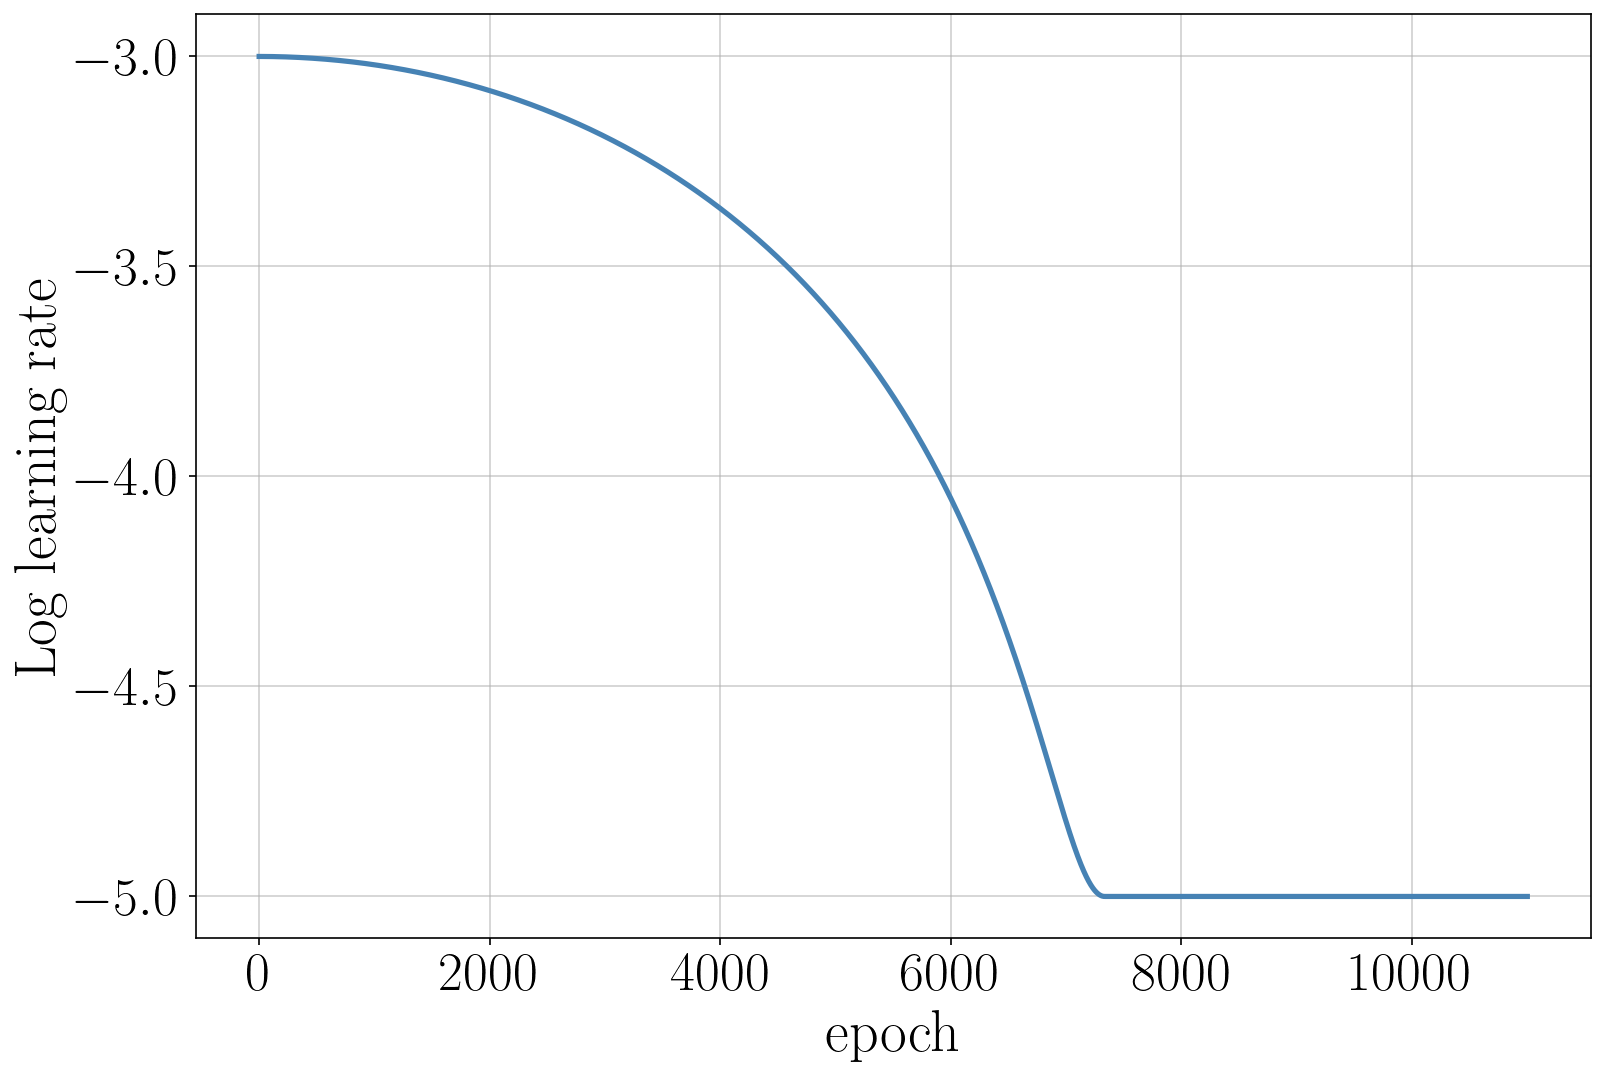
\includegraphics[width=0.6\linewidth]{figures/network_setup/lr}
	\caption{The evolution of the learning rate with each epoch on a logarithmic scale.}
	\label{fig:lr}
\end{figure}
